\begin{table}[p]
   \centering
   \footnotesize
   \renewcommand{\arraystretch}{1.15}
   \begin{tabular}{@{}>{\centering\arraybackslash}m{0.3033\textwidth}>{\centering\arraybackslash}m{0.3033\textwidth}>{\centering\arraybackslash}m{0.3033\textwidth}@{}}
      \hline
      \multicolumn{3}{@{}c@{}}{%
         \begin{tabular}{@{}>{\centering\arraybackslash}m{\dimexpr0.455\textwidth+\tabcolsep\relax}>{\centering\arraybackslash}m{\dimexpr0.455\textwidth+\tabcolsep\relax}@{}}
            $G_7$ & Matriz de adyacencia \\
            \hline
            \noalign{\vspace{6pt}}
            \rule{0pt}{0pt}$\vcenter{\hbox{\resizebox{0.45\textwidth}{!}{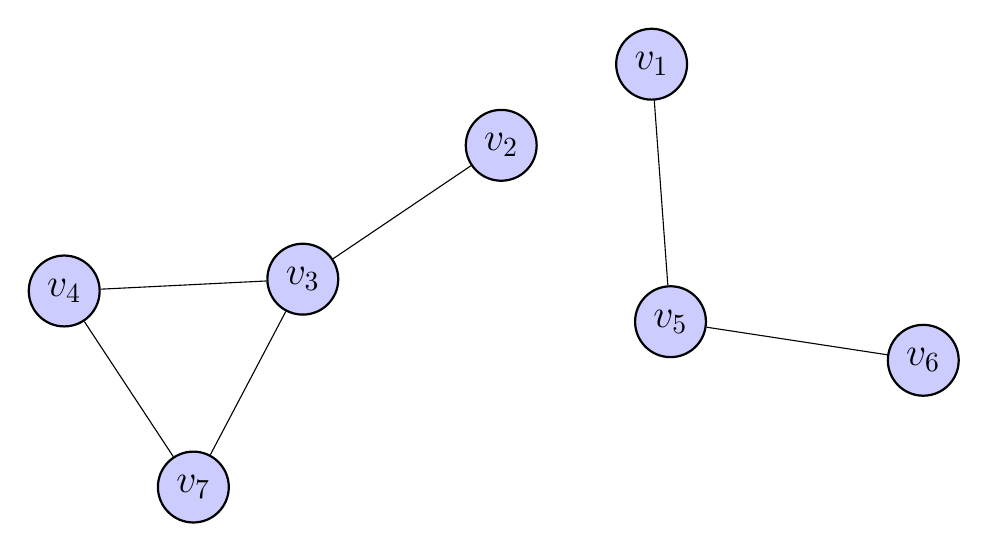
\begin{tikzpicture}[
  scale=1,
  vnode/.style={circle, fill=blue!20, draw=black, thick, minimum size=9mm, inner sep=0pt, font=\Large}
]
  % Vértices
  \node[vnode] (v1) at (7.85, 6.82) {$v_1$};
  \node[vnode] (v2) at (5.94, 5.79) {$v_2$};
  \node[vnode] (v3) at (3.42, 4.09) {$v_3$};
  \node[vnode] (v4) at (0.39, 3.94) {$v_4$};
  \node[vnode] (v5) at (8.09, 3.55) {$v_5$};
  \node[vnode] (v6) at (11.30, 3.06) {$v_6$};
  \node[vnode] (v7) at (2.03, 1.45) {$v_7$};

  % Aristas
  \foreach \from/\to in {v1/v5, v2/v3, v3/v4, v3/v7, v4/v7, v5/v6}
    \draw (\from) -- (\to);
\end{tikzpicture}
}}}$
            &
            $\vcenter{\hbox{$\begin{pmatrix}
         0 & 0 & 0 & 0 & 1 & 0 & 0 \\
         0 & 0 & 1 & 0 & 0 & 0 & 0 \\
         0 & 1 & 0 & 1 & 0 & 0 & 1 \\
         0 & 0 & 1 & 0 & 0 & 0 & 1 \\
         1 & 0 & 0 & 0 & 0 & 1 & 0 \\
         0 & 0 & 0 & 0 & 1 & 0 & 0 \\
         0 & 0 & 1 & 1 & 0 & 0 & 0
      \end{pmatrix}$}}$ \\
            \noalign{\vspace{6pt}}
         \end{tabular}%
      } \\
      \hline
      \multicolumn{3}{c}{\textbf{Topología de adyacencia}} \\
      \hline
      Abiertos subbásicos & Vecindades mínimas & Topología \\
      \hline
         ${A_{v_1}=\{v_5\}}$\par
         ${A_{v_2}=\{v_3\}}$\par
         ${A_{v_3}=\{v_2,v_4,v_7\}}$\par
         ${A_{v_4}=\{v_3,v_7\}}$\par
         ${A_{v_5}=\{v_1,v_6\}}$\par
         ${A_{v_6}=\{v_5\}}$\par
         ${A_{v_7}=\{v_3,v_4\}}$
      &
         ${U_{v_1}=\{v_1,v_6\}}$\par
         ${U_{v_2}=\{v_2,v_4,v_7\}}$\par
         ${U_{v_3}=\{v_3\}}$\par
         ${U_{v_4}=\{v_4\}}$\par
         ${U_{v_5}=\{v_5\}}$\par
         ${U_{v_6}=\{v_1,v_6\}}$\par
         ${U_{v_7}=\{v_7\}}$
      &
         No discreta, con 40 abiertos \\[6pt]
      \hline
      \multicolumn{3}{c}{\textbf{Topología de incidencia}} \\
      \hline
      Abiertos subbásicos & Vecindades mínimas & Topología \\
      \hline
         ${e_{1}=\{v_1,v_5\}}$\par
         ${e_{2}=\{v_2,v_3\}}$\par
         ${e_{3}=\{v_3,v_4\}}$\par
         ${e_{4}=\{v_3,v_7\}}$\par
         ${e_{5}=\{v_4,v_7\}}$\par
         ${e_{6}=\{v_5,v_6\}}$
      &
         ${U_{v_1}=\{v_1,v_5\}}$\par
         ${U_{v_2}=\{v_2,v_3\}}$\par
         ${U_{v_3}=\{v_3\}}$\par
         ${U_{v_4}=\{v_4\}}$\par
         ${U_{v_5}=\{v_5\}}$\par
         ${U_{v_6}=\{v_5,v_6\}}$\par
         ${U_{v_7}=\{v_7\}}$
      &
         No discreta, con 60 abiertos \\[6pt]
      \hline
   \end{tabular}
   \caption{Topologías de adyacencia e incidencia de $G_7$}
   \label{tab:topologias_G_7}
\end{table}
